\section{Theory}
\subsection{TMDC/Crystal structure}
\subsubsection{Transition metal dichalcogenides}
Transition metal dichalcogenides or TMDCs are a family of materials consisting of transition metals (group 3 through 12 on the periodic table) and chalcogen atoms (Sulphur, Selenium or Tellurium) in an \ce{MX_2}-configuration, where \ce{M} is the metal atom and \ce{X_2} are the chalcogen atoms \cite{C7TA04268J}.
The properties of TMDCs depend greatly on the amount of stacked layers and with individual layers being as thin as \SI{6.5}{\angstrom} for \ce{MoS_2} these materials are often referred to as layered or two-dimensional materials.
Decreasing the amount of layers from bulk changes electrical properties such as the bandgap which for some TMDCs can go from an indirect to a direct bandgap.
These electrical properties make TMDCs useful in electronics as transistors and in optoelectronics as emitters and detectors \cite{emerg_photolum, LopezSanchez2013, Radisavljevic2011}. 
If present, multiple layers of TMDCs are held together by weak interlayer Van der Waals forces making these materials flexible and transferable using polymer based techniques \cite{reganEmergingExcitonPhysics2022a}.

\subsubsection{Crystal lattice and band structure}
An infinitely repeating group of atoms is called an ideal crystal, such a crystal is constructed by attaching the same group of atoms, often called a unit cell, to a lattice.
The lattice can be constructed from $n$ independent lattice vectors. $n=1$ for an atomic chain, $n=2$ for a two-dimensional monolayer, and, $n=3$ for a three-dimensional crystal.
If no smaller repeating group of atoms can be constructed to fill the lattice then this group of atoms is called the primitive unit cell and the $n$-independent lattice vectors are then called the primitive translation vectors $a_{n}$ \cite{Kittel1995-qt}.
Each of the $n$ lattice vectors signifies a direction and length of displacement needed such that the shifted crystal lattice is indistinguishable from the original crystal lattice \ref{eq:lattice_equivalent}.
Lattice vectors are also used to specify the orientation of a crystal plane by denoting where the plane intersects the lattice vectors, this procedure allows for unique indexing of crystallographic planes. The use of these planes will be discussed in \ref{sec:diffraction}.
\begin{equation}
    \vec{r}' = \vec{r} + u_1 \vec{a_1} +u_2 \vec{a_2} + u_3 \vec{a_3}
    \label{eq:lattice_equivalent}
\end{equation}

\subsubsection{Reciprocal lattice and electron diffraction}
\label{sec:diffraction}
In the previous section the crystal lattice was introduced, and it was mentioned that there were unique planes characterized by the points where they intersect the lattice vectors.
In reciprocal space every lattice point is equivalent to one set of these planes.
To best understand a crystal, it is helpful to conceptualize it as having two lattices. The first lattice pertains to the organization of the atoms within the crystal's unit cells. The second lattice is a pattern of points that is specific to each crystal and does not correspond to the atom arrangement. Rather, each point in the lattice is linked to a particular set of planes within the crystal \cite{Williams2009-ww}.
Both lattice constructions are equally valid but are helpful under different circumstances; the reciprocal lattice, for instance, is a useful geometrical construct when talking about diffraction.

The reciprocal lattice, just like the crystal lattice, is constructed by vectors; in the case for the reciprocal lattice these are the reciprocal lattice vectors $\vec{b}_n$.
The reciprocal lattice vectors are constructed from the real-space lattice vectors using equation (\ref{eq:lattice_ortho_norm}) and satisfy relation (\ref{eq:lattice_vec_prop}) with their real-space counterpart.
Using these definitions the reciprocal lattice vectors are unique.
Any reciprocal vector can now be composed uniquely by a linear combination of the reciprocal lattice vectors, such that any vector is scaled and summed. If the scalars are integers they are the miller indices and correspond to a crystallographic plane. \\
Scattering off of these planes shows as a series of high-intensity spots in a diffraction pattern image (Figure \ref{fig:diffraction_pattern}), such an image can be taken in the diffraction mode of a scanning transmission electron microscope (STEM). \\

\begin{minipage}{0.5\textwidth}
    \begin{equation}
        \vec{b}_i = 2 \pi \vec{a}_j \times \vec{a}_k \cdot \left[ \vec{a}_i \cdot ( \vec{a}_j \times \vec{a}_k ) \right]^{-1} 
        \label{eq:lattice_ortho_norm}
    \end{equation}
\end{minipage}%
\begin{minipage}{0.5\textwidth}
    \begin{equation}
        \vec{b}_i \cdot \vec{a}_j = 2\pi \delta_{ij}
        \label{eq:lattice_vec_prop}
    \end{equation}
\end{minipage}\\

In a transmission electron microscope the electrons emanating from the field emission gun are modelled as plane waves. When incident on an atomically thin crystalline sample, the plane waves scatter predictably following the physical criteria that incoming and outgoing electrons beams are plane waves with wave vectors $\vec{k_I}$ and $\vec{k_O}$ for incoming and outgoing waves. The resulting change in wave vector due to the scattering of the sample is then equal to $\vec{K} = \vec{k_I}-\vec{k_O}$. As seen in Figure \ref{fig:scatt_angle}, the outgoing electron beam wavefront is deflected by an angle $\theta$ from the incident electron beam such that both are in phase, this angle is the Bragg angle \cite{Williams2009-ww}; and using that $\vert \vec{k_I} \vert = \vert \vec{k_O} \vert = \vert \vec{K} \vert =\lambda_e^{-1}$, with $\lambda_e$ the electron wavelength, the scattering angle can be expressed as:

\begin{equation}
    \sin{\theta}=\frac{\vert \vec{K}\vert / 2}{\vert \vec{k_I}\vert}
    \label{eq:bragg_angle}
\end{equation}

If both outgoing rays from the same incoming beam wavefront are then in phase, meaning that the extra distance travelled by on of the rays is a multiple of the wavelength, it shows as a bright spot in the image and then the following condition is met for the Bragg angle:

\begin{equation}
    n \lambda_e = 2 d \sin{\theta_B}
    \label{eq:bragg_angle_ser}
\end{equation}

This shows that scattering allows for a finite quantized momentum transfer from the electron to the crystal lattice or vice versa. In a crystalline sample this results in bright spots in the diffraction image, where each bright spot can be indexed and attributed to a family of planes in the crystal that facilitate the momentum transfer for the electrons to reach that spot on the detector or phosphor film.
Just as the real-space lattice has a unit cell so does the reciprocal lattice. In reciprocal space this unit cell is called the Brillouin zone.

\begin{figure}
    \centering
    
\includegraphics[width=0.3\textwidth, keepaspectratio]{resources/Figures/dp.png}
    \caption{Diffraction Pattern}
    \label{fig:diffraction_pattern}
\end{figure}

\begin{figure}
    \centering
    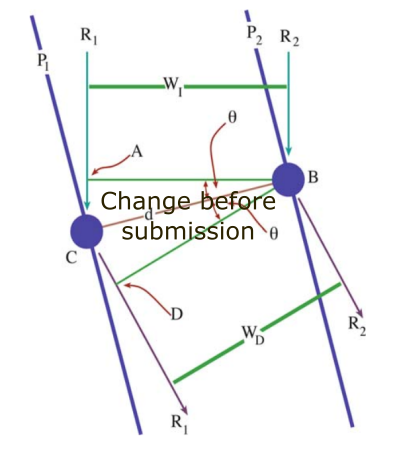
\includegraphics[width=0.3\textwidth, keepaspectratio]{resources/Figures/scattering.png}
    \caption{Scattering diagram}
    \label{fig:scatt_angle}
\end{figure}

\subsubsection{Convergent beam electron diffraction}



\subsection{Moiré Physics in two-dimensional heterostructures}
\begin{enumerate}
    \item moire pattern -> stacking
    \item lattice relaxation
    \item mini brillouin zone / aligned or antialigned
    \item hybridisation, inter/intra transistions and excitons
    \item band bending types, umklapp,  flat bands
\end{enumerate}


